TODO: Tree-fold Beispiele\\
Bestimme die Markierung lm links-Au\ss en im Baum t (oder \lstinline|empty| falls t leer ist).\footnote{Nach dem Prinzip von \glqq How to Replace Failure by a List of Successes \grqq, Wadler 1985}
\begin{minipage}[c]{0.25\textwidth}
t = \raisebox{-1cm}{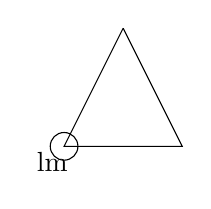
\begin{tikzpicture}
\draw(0,0)--(0.75,-1.5)--(-0.75,-1.5)--(0,0);
\draw (-0.75,-1.5) circle (5pt);
\node () at (-0.9,-1.7) {lm};
\end{tikzpicture}}
\end{minipage}%
\begin{minipage}[c]{0.75\textwidth}
\lstinline|(leftmost|\raisebox{-0.9cm}{\begin{tikzpicture}[->,>=stealth',level/.style={sibling distance = 1.25cm/#1,
  level distance = 1.25cm}] 
\node [arn_n] {x}
    child{ node [arn_x] {}                          
    }
    child{ node [arn_x] {}
		}
; 
\end{tikzpicture}}\lstinline|)| = \lstinline|(list x)|\\
\lstinline|(leftmost|\raisebox{-0.9cm}{\begin{tikzpicture}[->,>=stealth',level/.style={sibling distance = 1.25cm/#1,
  level distance = 1.25cm}] 
\node [arn_n] {x}
    child{ node [arn_t] {$\triangle$}                          
    }
    child{ node [arn_r] {?}
		}
; 
\end{tikzpicture}}\lstinline|)| = \lstinline[mathescape]|(leftmost $\triangle$)|
\end{minipage}
\begin{lstlisting}
(: leftmost (btree-of %a) -> (list-of %a))
(check-expect (leftmost empty-tree) empty)
(check-expect (leftmost t1) (list 1))
(check-expect (leftmost t2) (list 2))
(define leftmost
  (lambda (t)
    (btee-fold
      empty
      (lambda (l1 x l2)
        (if (empty? l1)
          (list x)
          l1))
      t)))
\end{lstlisting}
\begin{figure}[h!]
\centering
\begin{minipage}{0.75\textwidth}
\begin{minipage}{0.475\textwidth}
\begin{tikzpicture}
\draw[black,solid] (0,0)--(0,1);
\draw[black,solid] (0,0)--(1,0);
\draw[black,solid] (0,1)--(1,1);
\draw[black,solid] (1,1)--(1,0);
\draw[black,solid] (0.5,1)--(0.5,0);
\node () at (0.25,0.5) {$x_1$};
\draw[black,solid] (0.75,0.5)--(1.5,-0.75);
\draw[black,solid] (1.5,-0.75)--(1.5,-1.75);
\draw[black,solid] (1.5,-0.75)--(2.5,-0.75);
\draw[black,solid] (1.5,-1.75)--(2.5,-1.75);
\draw[black,solid] (2.5,-1.75)--(2.5,-0.75);
\draw[black,solid] (2.0,-1.75)--(2.0,-0.75);
\node () at (1.75,-1.25) {$x_2$};
\draw[black] (2.25,-1.25)--(3,-2.5);
\draw (3,-2.5)rectangle(4,-3.5);
\draw[black,solid] (3.5,-2.5)--(3.5,-3.5);
\node () at (3.85,-3.5) {\begin{rotate}{90}
\lstinline!empty!
\end{rotate}};
\node () at (3.25,-3) {$x_3$};
\end{tikzpicture}
\end{minipage}
\begin{minipage}{0.05\textwidth}
$\rightarrow\\
\leftarrow$
\end{minipage}
\begin{minipage}{0.475\textwidth}
\begin{tikzpicture}[->,>=stealth',level/.style={sibling distance = 3cm/#1,
  level distance = 1.5cm}] 
\node [arn_r] {1}
    child{ node [arn_x] {}                            
    }
    child{ node [arn_r] {2}
            child{ node [arn_x] {} 
            }
            child{ node [arn_r] {3}
							child{ node [arn_x] {}}
							child{ node [arn_x] {}}
            }
		}
; 
\end{tikzpicture}
\end{minipage}
\end{minipage}%
\begin{minipage}{0.25\textwidth}
Listen und rechtstiefe Bäume sind isomorph
\end{minipage}
\end{figure}
TODO: Grusts code hierzu\\
Ein \emph{Tiefendurchlauf} (\lstinline|depth-first-traversal|) eines Baumes t sammelt die Markierungen der Teilbäume l, r des Knotens.\\
$n = $\lstinline|make-node l x r| werden \emph{vor} x eingesammelt (Durchlauf zuerst in der Tiefe). Je nachdem ob x:\\
(a) zwischen, (b) vor, (c) nach den Markierungen von l,r eingezeichnet wird, erhält man einen
\begin{enumerate}[(a)]
\item \emph{inorder} traversal \qquad \ding{182}\ding{183}\ding{184}
\item \emph{preorder} traversal \qquad \ding{183}\ding{182}\ding{184} 
\item \emph{postorder} traversal \qquad \ding{182}\ding{184}\ding{183}
\end{enumerate}
\begin{lstlisting}[literate={}]
(: inorder ((btree-of %a) -> (list-of %a)))
(define inorder
  (lambda (t)
    (btree-fold
      empty
      (lambda (xs1 x xs2)
        (append 
          xs1@\ding{182}@
          (list x)@\ding{183}@
          xs2))@\ding{184}@
      t)))
\end{lstlisting}
Ein \emph{Breitendurchlauf} (\lstinline|(breadth-first-traversal)|) eines Baumes t sammelt die Markierungen der Knoten ebenenweise von der Wurzel ausgehend auf.\\
t $\equiv$ \begin{minipage}[c]{0.9\textwidth}
\begin{tikzpicture}[->,>=stealth',level/.style={sibling distance = 3cm/#1,
  level distance = 1.5cm}] 
\node [arn_r] {s}
    child{ node [arn_r] {c}
	    child{ node [arn_x] {}}
	    child{ node [arn_r] {e}
			child{ node [arn_x] {}}
			child{ node [arn_x] {}}}
    }
    child{ node [arn_r] {h}
		child{ node [arn_r] {m}
			child{ node [arn_x] {}}
			child{ node [arn_x] {}}}
		child{ node [arn_r] {e}
			child{ node [arn_x] {}}
			child{ node [arn_x] {}}}
            }
; 
\end{tikzpicture}
\end{minipage}\bigskip\\
\lstinline|(levelorder t)| \eval \lstinline|(list "s" "c" "h" "e" "m" "e")|\\
Idee: Gegeben sei eine Liste von Bäumen
\begin{enumerate}[(1)]
\item Sammle die Liste der Markierungen der Wurzeln der nicht leeren Bäume in ts auf \lstinline|(roots ts)|
\item Bestimme Liste ts' der nicht leeren Teilbäume der Bäume in ts \lstinline|(subtrees ts)|
\item Führe (1) rekursiv auf ts' aus
\item Konkateniere die Listen aus (1) und (3)
\end{enumerate}